\documentclass[12pt]{amsart}
\usepackage{amsmath,amssymb,url}
\usepackage{geometry} % see geometry.pdf on how to lay out the page. There's lots.
\geometry{a4paper} % or letter or a5paper or ... etc
% \geometry{landscape} % rotated page geometry

%  POSSIBLY USEFULE PACKAGES
%\usepackage{graphicx}
%\usepackage{tensor}
\usepackage{todonotes}
\usepackage{hyperref}

%  NEW COMMANDS
\newcommand{\pder}[2]{\ensuremath{\frac{ \partial #1}{\partial #2}}}
\newcommand{\ppder}[3]{\ensuremath{\frac{\partial^2 #1}{\partial
      #2 \partial #3} } }
\newcommand{\R}{\ensuremath{\mathbb{R}}}

%  NEW THEOREM ENVIRONMENTS
\newtheorem{thm}{Theorem}[section]
\newtheorem{prop}[thm]{Proposition}
\newtheorem{cor}[thm]{Corollary}
\newtheorem{lem}[thm]{Lemma}
\newtheorem{defn}[thm]{Definition}

%  NEW REMARKS
\theoremstyle{remark}
\newtheorem{rmk}[thm]{Remark}


%%%%%%%%%%%%%%% Holm Macros
\def\MM#1{\boldsymbol{#1}}
\newcommand{\pp}[2]{\frac{\partial #1}{\partial #2}} 
\newcommand{\dede}[2]{\frac{\delta #1}{\delta #2}}
\newcommand{\dd}[2]{\frac{\diff #1}{\diff #2}} 
\newcommand{\sothree}{\mathfrak{so}(3)}
% \contract is a differential geometry contraction sign _|
\def\contract{\makebox[1.2em][c]{\mbox{\rule{.6em}
{.01truein}\rule{.01truein}{.6em}}}}
%%%%%%%%%%%%%%%%%%%%%%%%%%%%%%%%%%%%%%%%%%%

%  MATH OPERATORS
\DeclareMathOperator{\SDiff}{SDiff}
\DeclareMathOperator{\GL}{GL}
\DeclareMathOperator{\SO}{SO}
\DeclareMathOperator{\ad}{ad}
\DeclareMathOperator{\Ad}{Ad}
\DeclareMathOperator{\Jet}{Jet}
\DeclareMathOperator{\Orb}{Orb}

%  TITLE, AUTHOR, DATE
\title{Jet vortex methods}
\author{Darryl D. Holm \& Henry O. Jacobs}
\date{\today}


\begin{document}

\begin{abstract}
A new singular vortex theory is presented for regularised Euler fluid equations of ideal incompressible flow in the plane. We determine the conditions under which such regularised Euler fluid equations may admit vorticity singularities which are stronger than delta functions, e.g., derivatives of delta functions. We also characterise the Hamiltonian dynamics of the higher-order singular vortices. Applications to the design of numerical methods similar to vortex blob methods are also discussed. 
\end{abstract}

\maketitle

\section{Introduction}
\label{sec:intro}
Consider the vorticity-stream formulation of an ideal incompressible planar fluid
\begin{align}
  \partial_t \omega + \partial_x \omega  \partial_y \psi
  - \partial_y \omega \partial_x \psi = 0. \label{eq:vorticity}
\end{align}
where $\omega = \Delta \psi$ is the vorticity and $\psi$ is the stream function.
The $(x,y)$ components of the Eulerian velocity field are given by
\begin{align*}
	(u,v) = (\partial_y \psi , - \partial_x \psi).
\end{align*}
If one is willing to view $\omega$ as a distribution, one can consider point vortex solutions.
In particular, point vortices are obtained if one considers the point vortex ansatz $\omega = \sum_{i} \Gamma_i \delta_{z_i}$
where $\Gamma_i \in \mathbb{R}$ and $\delta_{z_i}$ is the Dirac delta distribution centered at the point $z_i = (x_i,y_i) \in \mathbb{R}^2$.
Substitution of this ansatz into \eqref{eq:vorticity} yields the finite dimensional system
\begin{align}
\begin{cases}
	\frac{d \Gamma}{dt} = 0 \quad , \quad \psi(z) = \sum_i  \Gamma_i G(z-z_i) \\
	\frac{dx_i}{dt} = \partial_y \psi(z_i) \quad , \quad \frac{dy_i}{dt} = - \partial_x \psi(z_i)
\end{cases} \label{eq:point_vortex},
\end{align}
where $G(z) =  - (2\pi)^{-1} \ln( \| z \|)$.\todo{Should be be using $z$'s as shorthand for $(x,y) \in \R^2$}
One could consider the regularized form of the vorticity equation given by
choosing a translationally and rotationally invariant smoothing kernel $K_\delta$ and defining the regularized vorticity by 
$K_\delta* \omega = \Delta \psi$.
For example, $K_\delta (z) = \exp( - \| z\|^2 / \delta^2)$ is considered in \cite{BealeMajda1985}.
In this case the point vortex ansatz yields \eqref{eq:point_vortex} again, except $G$ is replace by
the kernel
\begin{align}
	G_\delta(z) := K_\delta*G(z) = \frac{1}{4\pi} \left( {\rm Ei}(- \| z \|^2 / \delta^2) - 2\ln ( \| z \|) \right). \label{eq:kernel}
\end{align}
where ${\rm Ei}( \cdot )$ denotes the exponential $i$ function.
The vorticity kernel $G_\delta$ has no singularity at the origin for $\delta > 0$, and is known as a vortex blob.
This system is the starting point for the vortex blob method, introduced in \cite{Chorin1973} (albeit with a different regularization).

The economy of the vortex method derives itself from the hyper-local character of Dirac delta distributions,
and the fact that \eqref{eq:vorticity} keeps them hyperlocal (i.e. parametrized by position).
However, there are many distributions which are localized to a similar degree (e.g. $\partial_x \delta_{z_i}$).
In this article we study the more general ansatz $\omega = \sum_{i,m,n} \Gamma_i^{mn} \partial_x^m \partial_y^n \delta_{z_i}$.
We will find that this ansatz yields a closed finite dimensional system which generalizes vortex blobs.
We call these new carriers of vorticity \emph{jet vortices}.

\subsection{Main contributions}
\begin{enumerate}
        \item We provide the equations of motion for jet vortices as exact solutions to a regularized fluid equation (\S \ref{sec:EOM}).
        \item We show how the equations of motion for the moments form a closed system (remark \ref{rmk:moments}).
        \item We derive conserved quantities:  Energy, angular momentum, linear momentum (remark \ref{rmk:conserved} and Appendix \ref{sec:symmetries})
        \item We observe the manifestation of Kelvin's circulation theorem for jet-vortices (\S \ref{rmk:Kelvin}).
        \item We perform numerical experiments with small numbers of jet vortices at orders $0$, $1$, and $2$.
        \item We spectrally approximate an initial condition using jet-vortices and plot the convergence rate (\S \ref{sec:approximation}). 
        \item We illustrate the ability to ``group'' nearby jet vortices into a single jet-vortex of higher order.
        	This can be used to reduce the number of pairwise interactions (\S \ref{sec:grouping}).
        \item We provide the symplectic and Hamiltonian structure of jet vortices (\S \ref{sec:symplectic}).
\end{enumerate}

\section{Background}
\label{sec:background}
Vortex methods for fluid modeling predate the computer age, and can be found as early as  a 1931 paper concerning a ``line of discontinuity'' in planar fluid flow \cite{Rosenhead1931}.
That point vortices induce an infinite velocity at the location of the vortex cores caused great difficulties numerically and theoretically,
and the method did not become a competitive numerical method until the 1970s.
In particular, these problems related to singularities were overcome by regularizing the singular vortex kernel to form a \emph{vortex blob}.
Additionally, stochastic perturbations were included to model viscosity and the Kutta condition was invoked to create vorticity around boundaries \cite{Chorin1973}.
These three adjustments to the classical vortex method made the method of practical use for realistic fluid flow modeling.
In particular, blob regularization proved much more amenable to analysis and the convergence to solutions of the Navier-Stokes equations was proven in \cite{Hald1979}.
Stronger convergence rates were achieved by judicious choice of vortex kernels.
By convolving the singular vortex kernel with sums of Gaussian smoothing kernels yields a sequence of vortex blob kernels with faster and faster convergence rates.
In particular the convergence rate of the $m$th kernel was found to be spectral, and of order $h^{mq}$ for any $q \in (0,1)$ where $h = \delta^q$
is a grid-spacing parameter and $\delta > 0$ is a length scale associated to the smoothing kernel \cite{BealeMajda1982,BealeMajda1985}.

Simultaneously, the symplectic geometry of point vortices was clarified in \cite{MarsdenWeinstein1983}
by invoking Arnold's interpretation of ideal fluids \cite{Arnold1966}.
The findings of \cite{MarsdenWeinstein1983} were later corrected in \cite{GayBalmazVizman2012} to handle fluid flow on manifolds with nontrivial homology.
While this clarified the geometry of point vortices, vortex blobs were thought to be a numerical ``trick" which broke the geometric interpretation.
However, this thought was vanquished with the invention of the Euler-$\alpha$ model, a regularized model of ideal fluids with a small parameter $1 \gg \alpha > 0$ \cite{HolmMarsdenRatiu1998}.
In particular, vortex blob solutions associated to a specific kernel serve as \emph{exact} solutions to the Euler-$\alpha$ model \cite{OliverShkoller2001}.
The Euler-$\alpha$ kernel is different from the kernels used in \cite{Chorin1973} and \cite{BealeMajda1985}.
A comparison of the Euler-$\alpha$ kernel to the $m=1$ kernel of \cite{BealeMajda1985} is given in \cite{HolmNitschePutkaradze2006}.

While vortex blobs performed well, they did not capture much of the qualitative richness observed in vorticity field dynamics.
In particular, blobs of vorticity in real ideal fluids are known to change shape and deviate from initially circular distributions.
A numerical method is proposed in \cite{Rossi1997,Rossi2005} to capture these shape dynamics by adding
basis functions with non-trivial moments in the study of vortex merger (see for example \cite{MelanderZabuskyMcWilliams1998,DizesVerga2002,MeunierDizesLeweke2005}).
Another distinct model obtained by projection onto a Hermite basis is described in \cite{NagemSandriUminskyWayne2009}.
This projection yields a finite-dimensional systems which models the (truncated) moments of the vorticity of an ideal incompressible fluid.
The derivation of simplified combinatorial formulas invoked by the dynamics of this model were discovered in \cite{UminskyWayneBarbaro2010}
and made the method numerically tractable at a large number of moments.

\section{Equations of motion}
\label{sec:EOM}
In this section we derive the equations of motion for jet-vortices.

\subsection{0th order}
Consider the ansatz for the vorticity
\begin{align}
  \omega(t) = \sum_{i} \Gamma_i(t) \delta_{z_i(t)} \label{eq:ansatz 0}
\end{align}
for constants $\Gamma_i(t) \in \R$ for $i$ in some finite set $S$
and where the points $z_i \in \R^2$ are distinct.
The stream function is 
\begin{align*}
  \psi(z;t) = \sum_{i} \Gamma_i(t) G_\delta (z-z_i(t) )
\end{align*}
and consequently, the corresponding velocity field is given by
\begin{align}
\begin{cases}
  u(z;t) = \sum_{i} \Gamma_i(t) \partial_y G_\delta (z-z_i(t) ) \\
  v(z;t) = - \sum_{i} \Gamma_i(t) \partial_x G_\delta (z-z_i(t) )
\end{cases} \label{eq:u 0}
\end{align}

An image of the stream function and the velocity field induced by a single vortex is depicted in figure \ref{fig:zero}

\begin{figure}[h] %  figure placement: here, top, bottom, or page
   \centering
   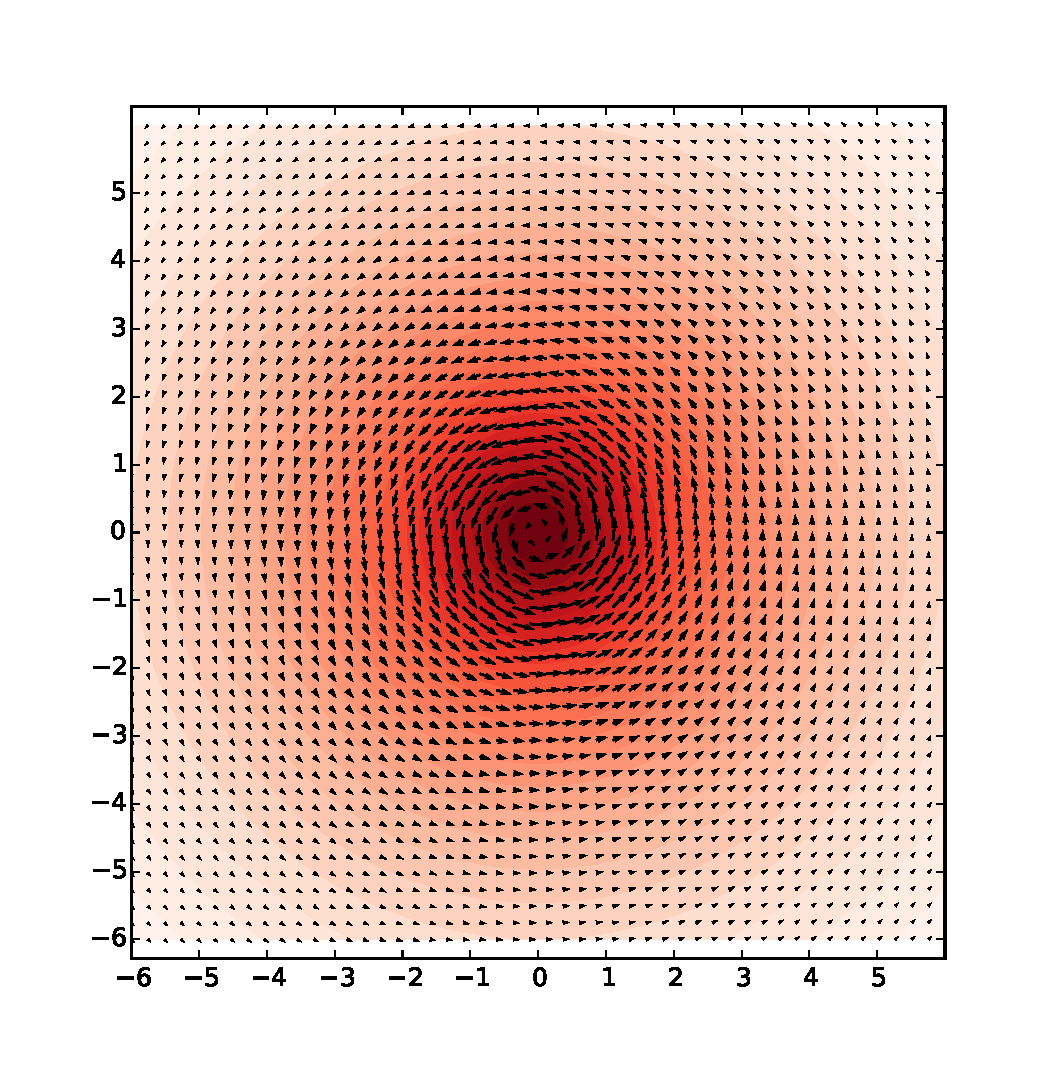
\includegraphics[clip,trim=0.6in 0.5in 0.6in 0.6in,width=0.6\textwidth]{./images/zero.pdf} 
   \caption{A 0th order jet vortex with $z = 0$ and $\Gamma=1$.
   With respect to the kernel $G_\delta$ of \eqref{eq:kernel}.
   By using vortices of this form we obtain one of the vortex blobs presented in \cite{BealeMajda1985}.}
   \label{fig:zero}
\end{figure}

We desire to find equations of motion for the $\Gamma_i(t)$'s and $z_i(t)$'s
such that the velocity field \eqref{eq:u 0} satisfies the vorticity equation \eqref{eq:vorticity}.
From this point on we will suppress the time dependence of all the quantities.

We then find
\begin{align}
  \partial_t \omega = \sum_{i} \frac{d \Gamma_i}{dt} \delta_{z_i} 
  - \Gamma_i \frac{dx_i}{dt} \partial_x \delta_{z_i}
  - \Gamma_i \frac{dy_i}{dt} \partial_y \delta_{z_i}.
  \label{eq:time derivative}
\end{align}
and
\begin{align*}
  u \partial_x \omega = \sum_{i} u \Gamma_i \partial_x \delta_{z_i}.
\end{align*}
Here $u \partial_x \delta$ should be interpreted
in terms of the basic theory of distrbutions.
Upon invoking \eqref{eq:func times partial delta} in Appendix
\ref{sec:distributions} we find
\begin{align}
  u \partial_x \omega = \sum_{i} \Gamma_i u(z_i) \partial_x \delta_{z_i} - \partial_x u(z_i) \delta_{z_i}. \label{eq:u term}
\end{align}
Similarly
\begin{align}
    v \partial_y \omega = \sum_{i} \Gamma_i v(z_i) \partial_y \delta_{z_i} - \partial_y v(z_i) \delta_{z_i}. \label{eq:v term}
\end{align}
Substituion of \eqref{eq:time derivative},\eqref{eq:u term},
and \eqref{eq:v term} into \eqref{eq:vorticity} yields
\begin{align*}
\frac{d \Gamma_i}{dt} \delta_{z_i} 
  - \Gamma_i \frac{dx_i}{dt} \partial_x \delta_{z_i}
  - \Gamma_i \frac{dy_i}{dt} \partial_y \delta_{z_i}
  + \Gamma_i u(z_i) \partial_x \delta_{z_i} - \partial_x u(z_i) \delta_{z_i}\\
  \quad + \Gamma_i v(z_i) \partial_y \delta_{z_i} - \partial_y v(z_i) \delta_{z_i} =  0.
\end{align*}
We observe this is a linear combination of the distributions $\delta_{z_i},\partial_x\delta_{z_i}$ and $\partial_y \delta_{z_i}$.
The coefficients of each must vanish independently.
The vanishing of the coefficient of $\delta_{z_i}$ yields
\begin{align*}
  \frac{d\Gamma_i}{dt} = \partial_x u(z_i) + \partial_y v(z_i).
\end{align*}
As the flow is divergence free we find
\begin{align*}
  \frac{d\Gamma_i}{dt} = 0.
\end{align*}
The vanishing of the coefficients $\partial_x \delta_{z_i}$ and $\partial_y \delta_{z_i}$ yields
\begin{align}
  \frac{dx_i}{dt} = u(z_i) \quad , \quad \frac{dy_i}{dt} = v(z_i).
  \label{eq:point motion}
\end{align}
Thus we have found equations of motion for $x_i(t),y_i(t)$ and $\Gamma_i(t)$
whose solutions make \eqref{eq:ansatz 0} into a solution of \eqref{eq:vorticity}.

\subsection{1st order}
Consider the first order jet-vortex ansatz for the vorticity
\begin{align}
  \omega(t) = \sum_{i} \Gamma_i(t) \delta_{z_i} 
  + \Gamma_i^x \partial_x \delta_{z_i}
  + \Gamma_i^y \partial_y \delta_{z_i}\label{eq:ansatz 1}
\end{align}
for constants $\Gamma_i(t),\Gamma_i^x(t),\Gamma_i^y(t) \in \R$ for $i = 1,\dots,N$.
The stream function is given by convolution
\begin{align*}
  &\psi(z;t) = G_\delta * \omega = \int G(z - \tilde{z}) \omega(\tilde{z}) d \tilde{z} \\
  &\quad = \sum_{i} \Gamma_i(t) G_\delta (z-z_i(t) )  + \Gamma_i^x(t) \partial_x G_\delta( z - z_i(t))  + \Gamma_i^y(t) \partial_y G_\delta( z- z_i(t))
\end{align*}
and so the corresponding velocity field is given by
\begin{align}
\begin{array}{ll}
  u(z;t) &= \sum_{i} \Gamma_i(t) \partial_yG_\delta (z-z_i(t) ) + \Gamma_i^x(t) \partial_{xy} G_\delta( z-z_i(t))\\
  &\qquad + \Gamma_i^y(t) \partial_y^2 G_\delta( z-z_i(t)) \\
  v(z;t) &= \sum_{i} -\Gamma_i(t) \partial_x G_\delta (z-z_i(t) ) - \Gamma_i^x(t) \partial_x^2 G_\delta( z-z_i(t)) \\
  &\qquad - \Gamma_i^y(t) \partial_{xy} G_\delta( z-z_i(t))
\end{array}
\label{eq:u 1}
\end{align}

\begin{figure}[h] %  figure placement: here, top, bottom, or page
   \centering
   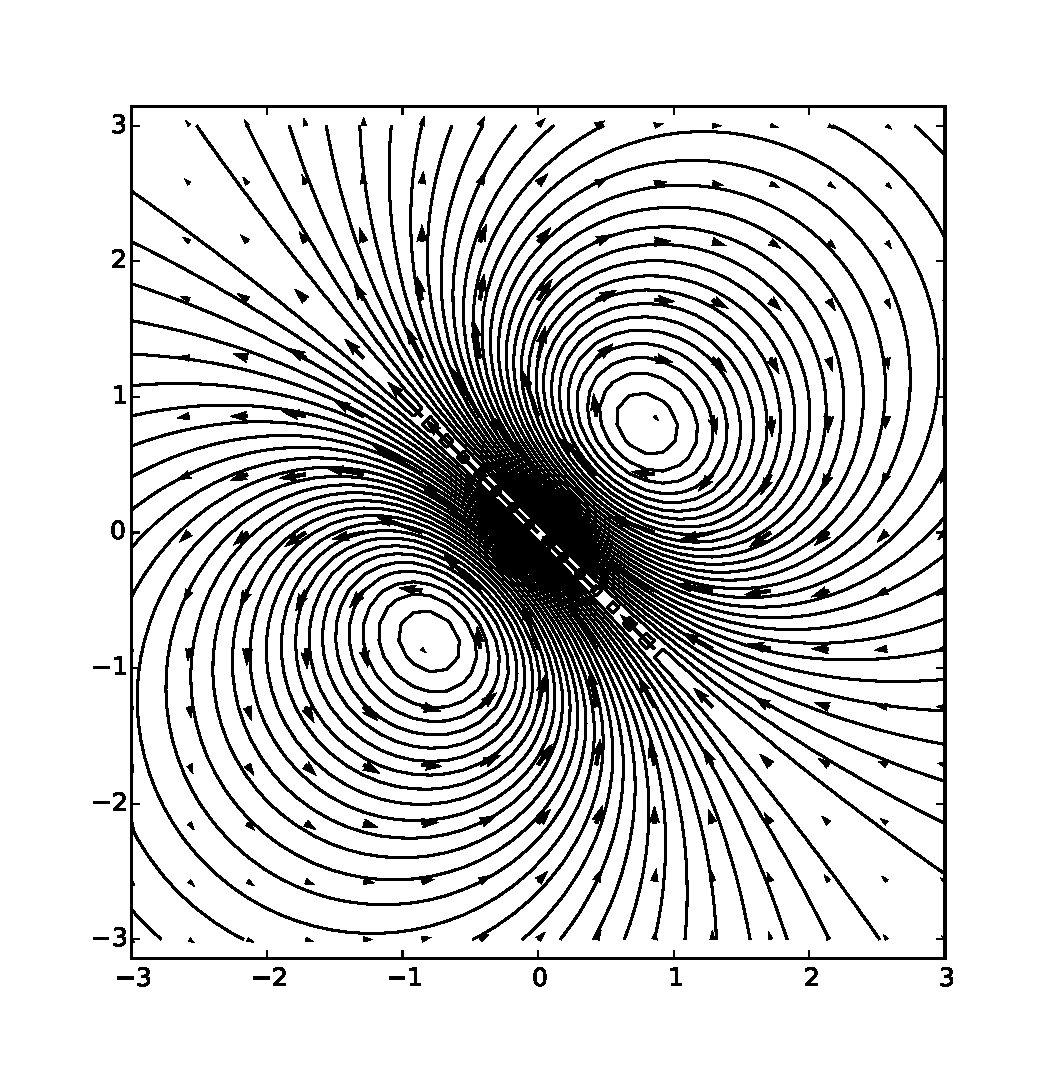
\includegraphics[clip,trim=0.6in 0.5in 0.6in 0.6in,width=0.6\textwidth]{./images/one.pdf} 
   \caption{A 1st order jet vortex with $\Gamma = 0,\Gamma^x = 1,\Gamma^y=1$.}
   \label{fig:one}
\end{figure}

We desire to find equations of motion for the $\Gamma_i(t)$'s and $z_i(t)$'s
such that the velocity field \eqref{eq:u 1} satisfies the vorticity equation \eqref{eq:vorticity}.
From this point on we will suppress the time dependence of all the quantities.
We then find
\begin{align*}
  \partial_t \omega = \sum_{i} & \frac{d \Gamma_i}{dt} \delta_{z_i} 
  - \Gamma_i \frac{dx_i}{dt} \partial_x \delta_{z_i}
  - \Gamma_i \frac{dy_i}{dt} \partial_y \delta_{z_i} \\
  &+\frac{d \Gamma_i^x}{dt} \partial_x\delta_{z_i} 
  - \Gamma_i^x \frac{dx_i}{dt} \partial_x^2 \delta_{z_i}
  - \Gamma_i^x \frac{dy_i}{dt} \partial_{xy} \delta_{z_i} \\
  &+\frac{d \Gamma_i^y}{dt} \partial_y \delta_{z_i} 
  - \Gamma_i^y \frac{dx_i}{dt} \partial_{xy} \delta_{z_i}
  - \Gamma_i^y \frac{dy_i}{dt} \partial_y^2 \delta_{z_i}
\end{align*}
and
\begin{align*}
  u \partial_x \omega = \sum_{i} u \Gamma_i \partial_x \delta_{z_i}
  + u \Gamma_i^x \partial_x^2 \delta_{z_i} 
  + u \Gamma_i^y \partial_{xy} \delta_{z_i}.
\end{align*}
Invoking \eqref{eq:func times partial delta} (see Appendix
\ref{sec:distributions}) we can revise the previous equation to
obtain
\begin{align*}
  u \partial_x \omega &= \sum_{i} \Gamma_i \Big( u(z_i) \partial_x \delta_{z_i} - \partial_x u(z_i) \delta_{z_i} \Big) \\
   &+\Gamma_i^x \Big(u(z_i) \partial_x^2 \delta_{z_i} 
   - 2\partial_x u(z_i) \partial_x \delta_{z_i}
   + \partial_x^2u(z_i) \delta_{z_i} \Big) \\
   &+\Gamma_i^y \Big( u(z_i) \partial_{xy} \delta_{z_i} 
   - \partial_x u(z_i) \partial_y \delta_{z_i} 
   - \partial_y u(z_i) \partial_x \delta_{z_i} 
   + \partial_{xy}u(z_i) \delta_{z_i}\Big)
\end{align*}
Similarly
\begin{align*}
    v \partial_y \omega &= \sum_{i} \Gamma_i \Big( v(z_i) \partial_y \delta_{z_i} - \partial_y v(z_i) \delta_{z_i} \Big) \\
   &\quad + \Gamma_i^x \Big(v(z_i) \partial_{xy} \delta_{z_i} 
   - \partial_x v(z_i) \partial_y \delta_{z_i}
   - \partial_y v(z_i) \partial_x \delta_{z_i}
   + \partial_{xy} v(z_i) \delta_{z_i} \Big) \\
   &\quad + \Gamma_i^y \Big( v(z_i) \partial_{y}^2 \delta_{z_i} 
   - 2\partial_y v(z_i) \partial_y \delta_{z_i} 
   + \partial_{y}^2v(z_i) \delta_{z_i} \Big)
\end{align*}
Substitution of these expressions into \eqref{eq:vorticity} yields
the vanishing of
a linear combination of the distributions
$\delta_{z_i},\partial_x\delta_{z_i},\partial_y \delta_{z_i}, \partial_x^2 \delta_{z_i},
 \partial_{xy} \delta_{z_i}$, and $\partial_y^2 \delta_{z_i}$.
As each of these distributions is linearly independent
of the others (assuming the $z_i$'s are distinct)
we find that the coefficients must vanish independently.
The vanishing of the coefficient of $\delta_{z_i}$ yields
the equation
\begin{align*}
  \frac{d\Gamma_i}{dt} = \partial_x u(z_i) + \partial_y v(z_i)
  + \partial_x^2 u(z_i) + \partial_{xy} v(z_i)
  + \partial_{xy} u(z_i) + \partial_y^2 v(z_i)
\end{align*}
Again, as the flow is divergence free we find
\begin{align*}
  \frac{d\Gamma_i}{dt} = 0.
\end{align*}
The vanishing of the coefficients of $\partial_x^2 \delta_{z_i}$ yields
\begin{align*}
  \Gamma_i^x \left( u(z_i) - \frac{dx_i}{dt} \right) = 0.
\end{align*}
Similarly, by looking at the coefficient of $\partial_y^2 \delta_{z_i}$
we find
\begin{align*}
  \Gamma_i^y \left( v(z_i) - \frac{dy_i}{dt} \right) = 0.
\end{align*}
Assuming $\Gamma_i^x$ and $\Gamma_i^y$ are non-zero we
obtain \eqref{eq:point motion} again.\footnote{
  After we obtain dynamics under this assumption
  we may drop the assumption by continous extension.
  The resulting extension yields the $0$th order
  jet-vortex dynamics.
}

Finally, the vanishing of the coefficients $\partial_x \delta_{z_i}$ and $\partial_y \delta_{z_i}$ yields
\begin{align*}
  \frac{d\Gamma^x_i}{dt} = \Gamma_i^x \partial_x u(z_i) + \Gamma_i^y \partial_y u(z_i) \\
  \frac{d\Gamma^y_i}{dt} = \Gamma_i^x \partial_x v(z_i) + \Gamma_i^y \partial_y v(z_i)
\end{align*}
Thus we have found equations of motion for $x_i(t),y_i(t)$ and the
$\Gamma_i(t)$'s.
The solutions of this finite-dimensional ODE
will make the first order jet-vortex ansatz, \eqref{eq:ansatz 1},
into a solution of \eqref{eq:vorticity}.

\subsection{$N$th order}
Consider the $N$th order jet-vortex ansatz for the vorticity
\begin{align}
  \omega(t) = \sum_{i \in S} \sum_{m+n \leq N} \Gamma^{mn}_i(t) \partial_x^m \partial_y^n \delta_{z_i} \label{eq:ansatz N}
\end{align}
for constants $\Gamma^{mn}_i(t),\Gamma_i^x(t),\Gamma_i^y(t) \in \R$ for $i \in S$.
The stream function is 
\begin{align*}
  \psi(z;t) = \sum_{i, m+n \leq N} \Gamma^{mn}_i(t) \partial_x^m \partial_y^n G_\delta (z-z_i(t) )
\end{align*}
and so the corresponding velocity field is given by
\begin{align}
\begin{cases}
  u(z;t) = \sum_{i \in S,m+n \leq N} \Gamma^{mn}_i(t) \partial_x^m \partial_y^{n+1} G_\delta (z-z_i(t) ) \\
  v(z;t) = - \sum_{i \in S, m+n \leq N} \Gamma^{mn}_i(t) \partial_x^{m+1} \partial_y^n G_\delta (z-z_i(t) )
\end{cases} \label{eq:u N}
\end{align}

\begin{figure}[h] %  figure placement: here, top, bottom, or page
   \centering
   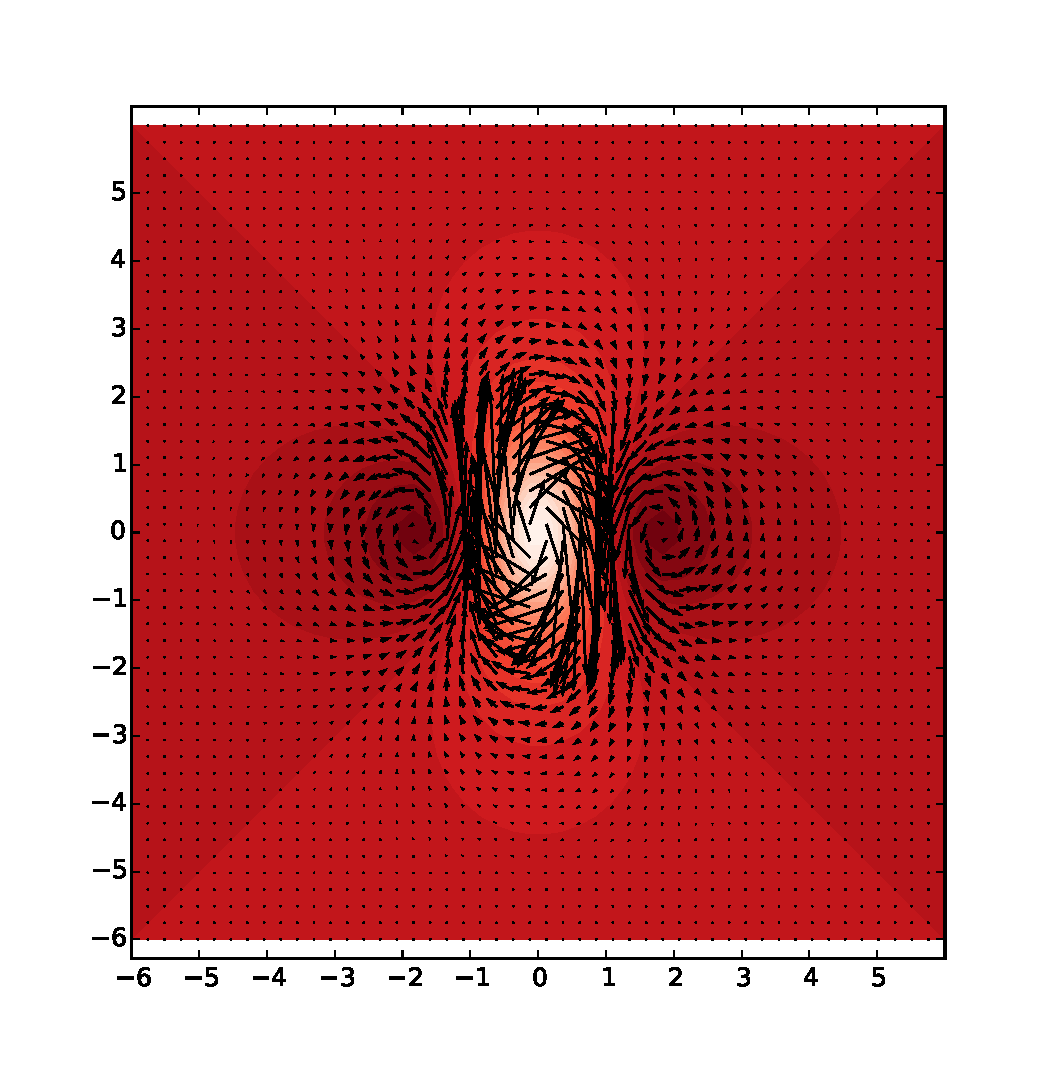
\includegraphics[clip,trim =1in 1in 1in 1in,width=0.3\textwidth]{./images/two_xx.pdf} 
   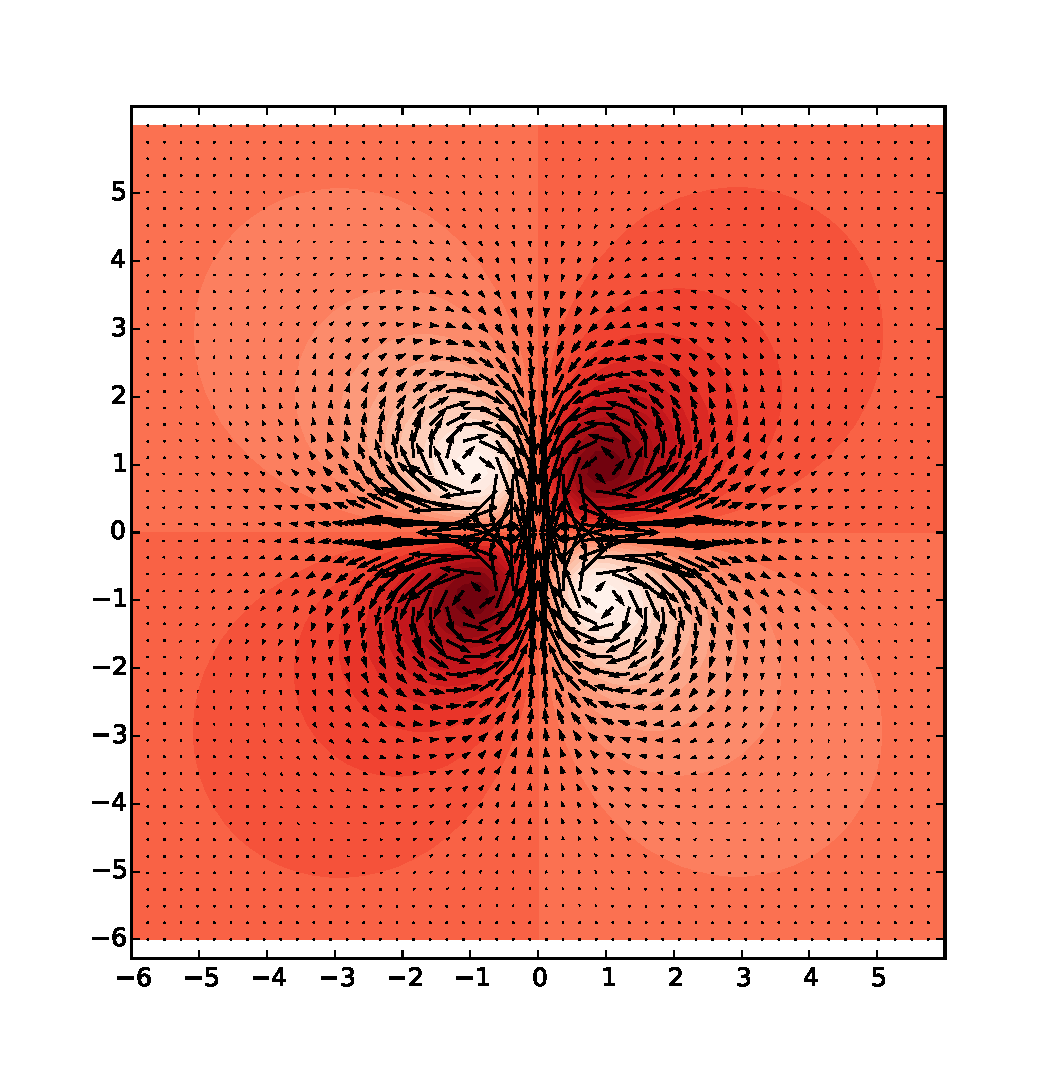
\includegraphics[clip,trim =1in 1in 1in 1in,width=0.3\textwidth]{./images/two_xy.pdf} 
   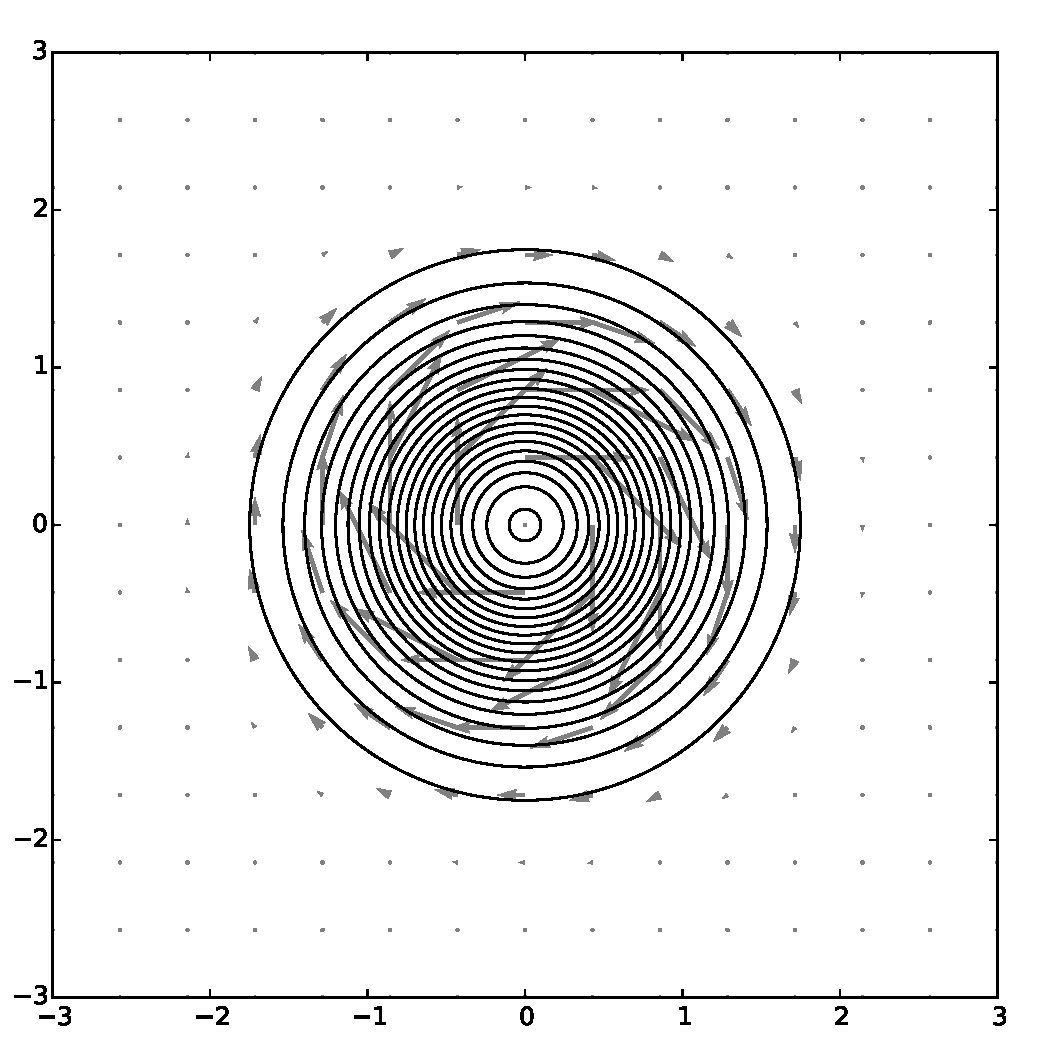
\includegraphics[clip,trim =1in 1in 1in 1in,width=0.3\textwidth]{./images/two_xx_yy.pdf} 
   \caption{Various second order jet vortices with $\Gamma^{00} = \Gamma^{1,0} = \Gamma^{0,1} = 0$.}
   \label{fig:second}
\end{figure}

We desire to find equations of motion for the $\Gamma^{mn}_i(t)$'s and $z_i(t)$'s
such that the velocity field \eqref{eq:u N} satisfies the vorticity equation \eqref{eq:vorticity}.
From this point on we will suppress the time dependence of all the quantities.


We then find
\begin{align*}
  \partial_t \omega =	
  \sum_{
  	\substack{
		i \in S \\
		m+n \leq N}}
  	\frac{d \Gamma_i^{mn}}{dt} \partial_x^m \partial_y^n \delta_{z_i} - \Gamma_i^{mn} \frac{dx_i}{dt} \partial_{x}^{m+1} \partial_y^{n} \delta_{z_i}
	- \Gamma_i^{mn} \frac{dy_i}{dt} \partial_{x}^{m} \partial_y^{n+1} \delta_{z_i}.
\end{align*}
and
\begin{align*}
  u \partial_x \omega = 
  \sum_{
  	\substack{
		i \in S \\
		m+n \leq N}}
   u \Gamma_i ^{mn}\partial_x^{m+1} \partial_y^n \delta_{z_i}.
\end{align*}
Invoking \eqref{eq:func times partial delta} (see Appendix
\ref{sec:distributions}) we can revise the previous equation to
obtain
\begin{align*}
  u \partial_x \omega &=
  \sum_{
  	\substack{
		i \in S \\
		m+n \leq N}}
	\Gamma_i^{mn} (-1)^{m+n+1} \sum_{\ell,k} (-1)^{\ell + k} \binom{m+1}{\ell} \binom{n}{k} \partial_x^{\ell} \partial_y^k u(z_i) \partial_x^{m+1-\ell} \partial_y^{n-k} \delta_{z_i}.
\end{align*}
Similarly
\begin{align*}
  v \partial_y \omega &=
  \sum_{
  	\substack{
		i \in S \\
		m+n \leq N}}
	\Gamma_i^{mn} (-1)^{m+n+1} \sum_{\ell,k} (-1)^{\ell + k} \binom{m}{\ell} \binom{n+1}{k} \partial_x^{\ell} \partial_y^k v(z_i) \partial_x^{m-\ell} \partial_y^{n+1-k} \delta_{z_i}.
\end{align*}
Substitution of these expressions into \eqref{eq:vorticity} yields
the vanishing of a linear combination of the distributions
$\partial_x^m \partial_y^n \delta_{z_i}$
for $m+n \leq N+1$.
As each of these distributions is linearly independent
of the others (assuming the $z_i$'s are distinct)
we find that the coefficients must vanish independently.
Assuming sufficiently many of the $\Gamma_i^{m,n}$'s are non-zero 
for $m+n = N$ we recover \eqref{eq:point motion}.\footnote{
  As before, after we obtain dynamics for the $\Gamma$'s under this assumption
  we may drop the assumption by continuous extension.
  The resulting extension yields the $0$th order
  jet-vortex dynamics.
}
The vanishing of the coefficient of $\delta_{z_i}$ yields
\begin{align*}
	\frac{d\Gamma^{0,0}_i}{dt} + \sum_{0 < m+n \leq N} \Gamma^{m,n} ( \partial_x^{m+1}\partial_y^n u(z_i) + \partial_x^{m}\partial_y^{n+1} v(z_i) ) = 0.
\end{align*}
As $u$ is divergence free this equation reduces to
\begin{align*}
	\frac{d \Gamma^{0,0} }{dt} = 0
\end{align*}

For $\ell+k \leq N$ the vanishing of the coefficient of $\partial_{\ell,k} \delta_{z_i}$ yields
\begin{align*}
  \dot{\Gamma}_i^{\ell k} = (-1)^{\ell + k}
  \sum_{
    \substack{
      m > \ell \\
      n > k \\
      n+m \leq p}
    }\Gamma_i^{mn} \Bigg[  \binom{n}{k} \binom{m}{\ell-1} \partial_{m-\ell+1,n-k} u^x(z_i) \\
   + \binom{n}{k-1} \binom{m}{\ell} \partial_{m-\ell,n-k+1} u^y(z_i)  \Bigg]
\end{align*}
Again, we have found equations of motion for $z_i(t)$'s and the
$\Gamma_i(t)$'s.
The solutions of this finite-dimensional ODE
will make the first order jet-vortex ansatz, \eqref{eq:ansatz 1},
into a solution of \eqref{eq:vorticity}.

\begin{rmk} \label{rmk:conserved}
  We will find that the following quantities are conserved:\\
  \begin{tabular}{|c|c|}
  	\hline
	  Linear momentum & $J_{lin} = \sum_i ( \Gamma_i^{0,1} - \Gamma^{0,0}_i y_i , \Gamma^{0,0}_i x_i -\Gamma^{1,0}_i )$ \\
	  \hline
	  Angular momentum & $J_{ang} = \sum_i \frac{\Gamma^{0,0}_i}{2} (x_i^2 + y_i^2) - \Gamma_i^{1,0} x_i - \Gamma_i^{0,1} y_i + \Gamma_i^{2,0} + \Gamma_i^{0,2}$ \\
	  \hline
	  Energy & $E = \sum_{m,n,\ell,k,i} (-1)^{m+n+\ell +k} \Gamma^{mn}_i \Gamma_j^{\ell k} \partial_{m+\ell}^x \partial_{n+k}^y G(z_i-z_j)$ \\
	  \hline
  \end{tabular}\\
  \todo[inline]{This table is too cramped.  Find a way to fix the spacing}
  The first two are momenta derived by observing the rotational and
  translational symmetry of the fluid and applying Noether's theorem.
  In section \ref{sec:symplectic} we will characterize fluids, and the jet-vortices as Hamiltonian systems
  and the Linear and angular momentum serve as symplectic momentum maps (see Appendix \ref{sec:symmetries} for derivation).
\end{rmk}

\begin{rmk} \label{rmk:Kelvin}
	Let $\vec{u}$ be a time-dependent vector field which satisfies \eqref{eq:vorticity}.
	The flow of $\vec{u}$ is the diffeomorphism, $\Phi_t: \mathbb{R}^2 \to \mathbb{R}^2$,
	which sends particle labels at time $0$ to their positions at time $t$.
	If $\omega_t$ is the vorticity at time $t$ then $\omega_t( \Phi_t(z) ) = \omega_0$ is constant in time.
	This conservation law can be seen as a corollary of Kelvin's circulation theorem.
	As a consequence,
	\begin{align*}
		J(t) := \int \omega_t( \Phi_t(z) ) f(z) dz
	\end{align*}
	is constant in time for any $f \in C^\infty(\R^2)$.
	By applying the change of variables formula and invoking the
	incompressibility condition, $\det(D\Phi) = 1$, we find
	\begin{align*}
		J(t) = \int \omega_t( z) f(\Phi_t^{-1}(z)) dz.
	\end{align*}
	This form of writing $J(t)$ makes sense when $\omega_t$ is a distribution.
	As a result, we find that for a vorticity of the form \eqref{eq:ansatz N} the quantity
	\begin{align}
		J(t) = \sum_{
			\substack{
				i \in S \\
				m+n \leq N
			}
		} \Gamma_i^{mn} (-1)^{m+n} \partial_x^m\partial_y^n( f \circ \Phi_t^{-1}) |_{z = z_i(t)} \label{eq:conserved_circulation}
	\end{align}
	is conserved for any $f \in C^\infty(\R^2)$.
	While this conservation law holds for all functions, $f$, we do not obtain infinitely many conserved
	quantities when $\omega_t$ satisfies the jet-vortex ansatz and $S$ is finite.
	This is because the expression on the right hand side only depends on the $N$-jet of $f$ at $z_i(0) \equiv \Phi_t^{-1}(z_i(t) )$,
	as is illustrated by the Fa\`a di Bruno formula.
	We will not display the Fa\`a di Bruno formula here because it requires nearly a page of notational definitions before to writing it down
	\cite{ConstantineSavits1996,Jacobs2014b}.
	Nonetheless, by computing the cardinality of jet spaces, we would obtain ${\rm card}(S) \frac{ N(N+1)}{2}$ independent conserved quantities
	as a result of \eqref{eq:conserved_circulation}.
	These conserved quantities can be interpreted as a finite dimensional manifestation of the conservation of circulation.
\end{rmk}

\begin{rmk}\label{rmk:moments}
	The $(a,b)^{\rm th}$ moment of the vorticity centered around the vortex position $(x_i,y_i) \in \R^2$ is given by
	\begin{align*}
		\mu^{ab}_i := \int (x-x_i)^a (y-y_i)^b \omega dxdy
	\end{align*}
	If $\omega$ satisfies the jet-vortex ansatz \eqref{eq:ansatz N} then
	\begin{align*}
		\mu^{ab}_i = \sum_{
			\substack{
				j \in S \\
				m \leq a ,
				n \leq b
			}
		}
		(-1)^{m+n} \frac{a! b!}{(a-m)!(b-n)!} \Gamma_j^{mn} (x_j - x_i)^{a-m} (y_j - y_i)^{b-n}
	\end{align*}
	for $a+b \leq N$ and $i \in S$.
	We see that given the points $z_i \in S$ we can write the moments in terms of the circulation
	strengths, the $\Gamma$'s.
	For the moment $\mu_i^{ab}$ with $a+b \leq N$ with $a,b \in \mathbb{N}$
	we may invert this relationship to write $\Gamma_i^{mn}$ as a function of these moments.
	Invoking the equation of motion for the $\Gamma$'s and substituting the identity be tween the $\Gamma$'s
	and the $\mu$'s
	would yield a closed dynamical system for the $\mu$'s.
	That the equations of motion for the moments forms a closed system at order $N$
	is in contrast to other methods for deriving dynamical systems for moments
	\cite{UminskyWayneBarbaro2010, NagemSandriUminskyWayne2009,GibbonsHolmTronci2008a,GibbonsHolmTronci2008b}
	where a projection must be invoked in order to form a closed system.
\end{rmk}

\section{Numerical Aspects}
\label{sec:numerics}
\todo[inline]{Write intro to numerics section}

\subsection{Convergence to Euler's}
\todo[inline]{Write this section}
This is basically proven already, as we can invoke the error bounds of BealeMajda.

\subsection{Grouping and reduction of pairwise computations}
\label{sec:grouping}

Let us consider the vorticity distribution
\begin{align*}
	\omega = \Gamma_1 \delta_{z_1} + \Gamma_2 \delta_{z_2}
\end{align*}
if $z_1$ and $z_2$ are close we can define the quantities $\bar{z} = (z_1+z_2)/2$ and $\delta z = z_1 - z_2 $ to obtain the approximation
\begin{align*}
	\int \omega(z) f(z)dz &= \Gamma_1 f(z_1) + \Gamma_2 f(z_2) \\
		&= \Gamma_1 \left( f(\bar{z}) + \partial_x f(\bar(z)) \cdot \frac{\delta x}{2} + \partial_y f(\bar(z)) \cdot \frac{\delta y}{2}  \right)\\
		&\quad + \Gamma_2 \left( f(\bar{z}) - \partial_x f(\bar(z)) \cdot \frac{\delta x}{2} - \partial_y f(\bar(z)) \cdot \frac{\delta y}{2}  \right) + o( h ) 
\end{align*}
where $h = \| \delta z \|$.
Therefore the distribution
\begin{align*}
	\tilde{\omega} = \Gamma \delta_{\bar{z}} + \Gamma^x \partial_x \delta_{\bar{z}} + \Gamma^y \partial_y \delta_{\bar{z}}
\end{align*}
with 
\begin{align*}
	\Gamma = \Gamma_1 + \Gamma_2 \quad,\quad \Gamma^x = \frac{\delta x}{2} (\Gamma_1 -\Gamma_1) \quad,\quad \Gamma^y = \frac{\delta y}{2} (\Gamma_1 -\Gamma_1)
\end{align*}
serves as a $o(h)$ approximation of $\omega$ in the sense of distributions.
Moreover, the stream function $\tilde{\psi} := G_\delta * \tilde{\omega}$ is an $o(h)$ approximation of $\psi := G_\delta * \omega$ in the traditional sense of analysis on functions.

What has just been described is the first case of grouping two $N$th order jet vortices concentrated at $z_1$ and $z_2$ into a single $(N+1)$th order jet vortex concentrated at 
the average position $\bar{z}$.
More generally, we can consider the ansatz
\begin{align*}
	\omega = \sum_{m+n \leq N} \Gamma_1^{mn} \partial_x^m \partial_y^n \delta_{z_1} + \Gamma_2^{mn} \partial_x^m \partial_y^n \delta_{z_2}
\end{align*}
and observe
\begin{align*}
	&\int \omega(z) f(z)dz = \sum_{m+n \leq N} (-1)^{m+n} \left( \Gamma_1^{mn} \partial_x^m \partial_y^n f(z_1) + \Gamma_2^{mn}  \partial_x^m \partial_y^n f(z_2) \right)\\
		&\quad= \Bigg\{ \sum_{m+n \leq N} (-1)^{m+n} \Gamma_1^{mn} \left( \partial_x^m \partial_y^n  f(\bar{z}) + \partial_x^{m+1} \partial_y^n  f(\bar(z)) \cdot \frac{\delta x}{2} + \partial_x^m \partial_y^{n+1} f(\bar(z)) \cdot \frac{\delta y}{2}  \right)\\
		&\qquad +  (-1)^{m+n} \Gamma_2^{mn} \left( \partial_x^m \partial_y^n  f(\bar{z}) - \partial_x^{m+1} \partial_y^n  f(\bar(z)) \cdot \frac{\delta x}{2} - \partial_x^m \partial_y^{n+1} f(\bar(z)) \cdot \frac{\delta y}{2}  \right) \Bigg\} \\
		&\qquad + o( h ) .
\end{align*}
The above computation implies that 
\begin{align*}
	&\tilde{\omega} :=\\
	 &\sum_{m+n \leq N+1} \left( \Gamma_1^{mn} + \Gamma_2^{mn}
	- \frac{\delta x}{2}( \Gamma_1^{ m-1,n} - \Gamma_2^{m-1,n} ) - \frac{\delta y}{2} ( \Gamma_1^{m,n-1} - \Gamma_2^{m,n-1}) \right) \partial_x^m \partial_y^n \delta_{\bar{z}}
\end{align*}
serves as an $o(h)$ approximation of $\omega$.
Of course, this again implies that the corresponding stream functions are approximated to order $h$ as well.
Note that $\tilde{\omega}$ is concentrated above a single point, $\bar{z}$, while $\omega$ is concentrated above two points.

\begin{rmk}
Such reductions are even more dramatic when considering higher order jets.
In particular, $2^N$ zeroth order jet vortices can be approximated with a single $N$th order jet vortex by applying the above approximations iteratively.

The computation of pairwise interactions in the vortex method was a primary bottleneck in implementing the standard vortex method for real-world applications.
It was not until the invention of the fast multipole method, that it became tractable to compute millions of pairwise interactions by
reducing the complexity from an $\mathcal{O}(n^2)$ calculation to an $\mathcal{O}(n \log (n))$ calculation, where $n$ is the number of vortices \cite{GreengardRokhlin1987}.
However, in the case of viscous fluids with boundaries, vorticity is shed from the boundaries.
As a result, the vortex blob method of \cite{Chorin1973} created new vortices at the boundary by using the Kutta condition as a creation criteria.
For these applications, $n$ will grow in time without bound, and some means of discarding vortices must be invoked.
It is here that the grouping of jet-vortices  could be useful.
If one mergers two $N$-jet vortices to obtained a $(N+1)$-jet vortex, the amount of scalars and data typically increases.
So one must still make a tough decision as to what data to discard (e.g. through some tolerance or simply truncating at level $M$).
Nonetheless, the analysis presented here could shed light on how best to implement this.
\end{rmk}

\begin{rmk}
The merging of blobs of vorticity has been studied analytically \cite{MelanderZabuskyMcWilliams1998},
numerically \cite{WeissMcWilliams1993,MelanderZabuskyMcWilliams1998,DizesVerga2002}
as well as in the lab \cite{FineDriscollMalmbergMitchell1991}.
All of this is in the lightly viscous (or nearly inviscid) regime.
Grouping can be used to numerically resolve such collision events.
In theory, there is no issue with collisions because we are considering regularized vortices where
the induced velocity field from a single jet-vortex is always finite.
However, as $\delta$ becomes smaller, the velocity near the vortex core diverges.
This should be of concern as the convergence analysis of the vortex method pre-supposes that $\delta \ll 1$.
Typically such a near collision is dealt with by using a smaller time-step (as the ODE is quite stiff).
Grouping of jet-vortices suggests an alternative by avoiding this pair-wise interaction altogether.
Perhaps such an approach could be viewed as a variation of the punctuated dissipation events
described in \cite{WeissMcWilliams1993} where an initial vorticity distribution is found to asymptotically
approach a smoother axisymmetric vortex blob,
and discrete vortex mergers are implemented to model this behavior.
\end{rmk}

\subsection{Approximation of initial conditions}
\label{sec:approximation}
In this section we will illustrate how using jet-vortices will increase the accuracy of approximation of a vorticity field in a distributional sense
with respect to a reproducing kernel Hilbert space (RKHS).
Let $H(\omega) = \frac{1}{2} \langle \omega , G*\omega\rangle_{L^2} =: \frac{1}{2} \langle \omega , \omega \rangle_G$, for a Green's kernel $G:\R^2 \to \R$.
Let $h > 0$ be small and define $h \mathbb{Z}^2 = \{ (ah,bh) \in \R^2 \mid (a,b) \in \mathbb{Z}^2 \}$.
Given an $\omega \in \mathcal{D}'(\R^2)$, we can attempt to approximate $\omega$ via Dirac-deltas supported on $h \mathbb{Z}^2$.
There is a natural way to do this with respect to the Hilbert-norm because we have a reproducing kernel.
We could define $\omega_h^{(0)} = \sum_{i \in \mathbb{Z}^2} \Gamma_i \delta_{z_i}$ by requiring the error, $\omega_h^{(0)} - \omega$, to be $\langle \cdot , \cdot \rangle_{G}$-orthogonal to $\delta_z$ for each $z \in h \mathbb{Z}^2$.
This means that $G*\omega(z) =  \sum_i \Gamma_i G(z-z_i)$ for each $z \in h\mathbb{Z}^2$.
Thus $\psi_h^{(0)} = \sum_i \Gamma_i G(z-z_i)$ can be seen as a $0$th order approximation to $\psi = G*\omega$
because $\psi_h^{(0)}(z) = \psi(z)$ for all $z \in h\mathbb{Z}$.
 
The same reasoning applies if we consider $\omega^{(k)}_h = \sum_{i,m+n \leq N} \Gamma_i^{mn} \partial_x^m \partial_y^n \delta_{z_i}$.
We define the scalars $\Gamma_i^{mn}$ via the equations
\begin{align*}
  \partial_x^\ell \partial_y^k \psi (z_i) = \sum_j (-1)^{m+n} \Gamma_j^{mn} \partial_x^{m+\ell} \partial_y^{n+k} G(z_i - z_j)
\end{align*}
for $\psi = G*\omega$, $z_i \in h \mathbb{Z}^2$, and $|\beta| \leq k$.
Then $\psi^{(k)}_h = \sum_{i,\alpha} (-1)^{m+n} \Gamma_k^{mn} \partial_x^m \partial_y^n G_{z_i}$
serves as an order $k$ approximation of $\psi$ when $\psi \in C^k$.

This is not to say that the convergence rate is simple $O(h^k)$.
The convergence of the initial condition, and in fact the full fluid system
upon integrating the equations of motion, is a spectral convergence.
Moreover, this spectral convergence rate of the full system relies heavily on the choice of kernel
\cite{BealeMajda1982}.

As an example we numerically compute the corresponding approximations of the stream function
\begin{align}
        \psi(x,y) = \exp( - r^2 ) - \exp( - r^2 / 2 )
        \label{eq:psi_exact}
\end{align}
The results are depicted in figure \ref{fig:convergence}.
As we are unable to grid all of $\mathbb{R}^2$, the error
is only measured on a small subregion ($-3<x<3, -3<y<3$) within the region covered by our grid
($-6<x<6, -6 < y < 6 $).
We observe the predicted spectral convergence using jet-vortices at orders zero, one, and two.
In each case, a grid spacing is reached where the convergence simply goes no further (possibly 
due to machine precision).
Nonetheless, higher order jet vortices appear to out perform lower order ones for smaller grid spacings.
\begin{figure}[h]
        \centering
        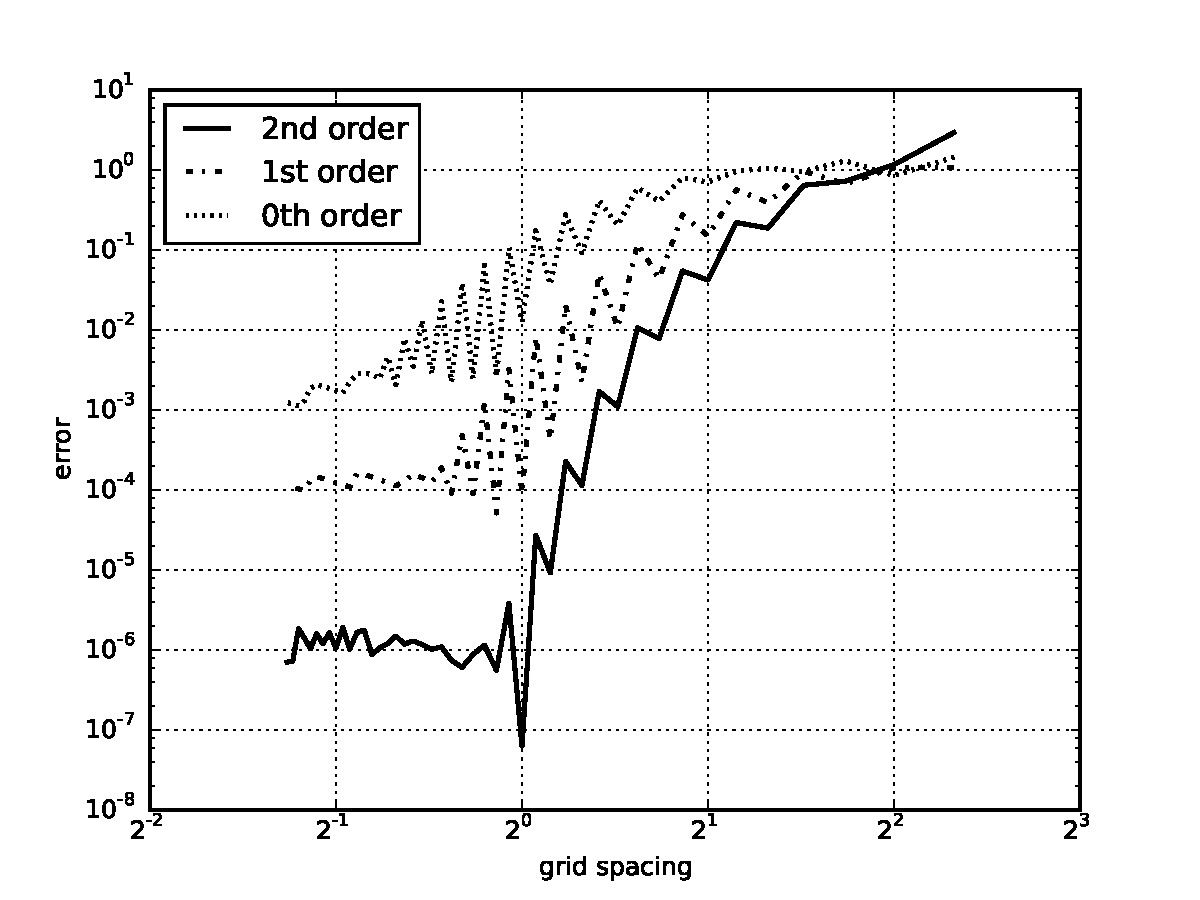
\includegraphics[width=0.7\textwidth]{./images/convergence.pdf}
        \caption{A convergence plot of the error in the sup-norm
        of the reconstructed stream function approximated with zeroth (blue),
        first (green), and second (red) order jet-vortices.
        The method converges spectrally, so no specific convergence rate is observed.}
        \label{fig:convergence}
\end{figure}

\subsection{Numerical experiments}
\label{sec:numerical_expirements}
\todo[inline]{Write numerical experiments section}

\section{Hamiltonians and symplectic structures}
\label{sec:symplectic}
In the modern conception of Hamiltonian mechanics, as described in \cite{FOM,Arnold2000},
the Hamiltonian is a function on a symplectic manifold, which produces equations of motion.
An important instance of a symplectic manifold is a coadjoint orbit.
In this section we compute the coadjoint orbit of a jet-vortex
as well as the associated symplectic structure.
For a general vorticity distribution $\omega$, the Hamiltonian is the kinetic energy
\begin{align*}
  H(\omega) = \frac{1}{2} \langle \omega , G_\delta* \omega \rangle.
\end{align*}
Where $\omega$ may be of the form \eqref{eq:ansatz N}.

The coadjoint orbit of $\omega$ is the set
\begin{align*}
  \Orb(\omega) := \{ \varphi_* \omega \mid \varphi \in \SDiff(\R^2) \}
\end{align*}
where $\varphi_* \omega$ denotes the distribution defined by
\begin{align*}
	\int f(z) (\varphi_*\omega)(z) := \int f(\varphi(z)) \omega(z) \quad , \quad \forall f \in C^\infty(\R^2).
\end{align*}
In fact $\Orb(\omega)$ inherits the structure of a smooth manifold,
and a tangent vector on $\Orb(\omega)$ at the point $\tilde{\omega} \in \Orb(\omega)$ is given by 
a distribution of the form $\pounds_{\vec{u}}[\tilde{\omega}] := u \partial_x \tilde{\omega} + v \partial_y \tilde{\omega}$ for some (non-unique) divergence free vector field
$\vec{u} = (u,v) \in \mathfrak{X}_{\rm div}(\R^2)$.
The symplectic structure is nothing more than a special case of one derived via the Kirillov-Kostant-Souriau theorem \cite[see the boxed formula on p.303]{FOM}.
In particular, the symplectic structure on $\Orb(\omega)$ is given by
\begin{align}
  \Omega_\omega( \pounds_{\vec{u}_1}[\omega] , \pounds_{\vec{u}_2}[\omega] ) = \int \omega(z)  ( u_1(z) v_2(z) - v_1(z) u_2(z) ) dz. \label{eq:symplectic}
\end{align}
In the case that $\omega$ is a smooth distribution, it may be identified with a differential $2$-form and this formula matches the symplectic form derived on page 313 of \cite{MarsdenWeinstein1983}.
In the case that $\omega$ satisfies the ansatz \eqref{eq:ansatz N}, we find that $\Orb(\omega)$ is finite dimensionally parametrizable in the following theorem.

\begin{thm}
	Let $\omega_0 = \gamma_i^\alpha \partial_{\alpha} \delta_{Z_i}$ for $\gamma_i^\alpha \neq 0$ and let
	$M^{(k)} = \{ \sum_{|\alpha| \leq k} \Gamma_i^\alpha \partial_{\alpha} \delta_{Z_i} \}$.
	Then $\Orb(\omega_0)$ is a sub-manifold of the $M^{(k)}$.
\end{thm}
\begin{proof}
	Let $\varphi \in \SDiff(\R^2)$.  Then
	\begin{align*}
		\langle \varphi_* \omega_0 , f \rangle &= \langle \omega_0 , f \circ \varphi \rangle \\
                &= \gamma_i^\alpha \partial_{\alpha}|_{z=Z_i} (f \circ\varphi)(z) \\
                &= \gamma_i^\alpha \partial_{\beta}|_{\varphi(Z_i)} f \partial_\beta|_{Z_i} \varphi^\alpha.
	\end{align*}
        Where we have used the Fa\`a di Bruno formula via the multi-indexing convention of \cite{Jacobs2014b}.
        Thus $\varphi_* \omega_0 \in M^{(k)}$.
\end{proof}

Finally, as a check, we can also prove that the equations of motion are identical to the equations of motion obtained using this symplectic structure.

\begin{thm}
	Let $H(\omega) = \frac{1}{2} \langle \omega , G*\omega \rangle_{L^2}$.  Then Hamilton's equations on $\Orb(\omega_0)$
	are given by
	\begin{align*}
		\partial_t \omega + \partial_y \psi \partial_x \omega - \partial_x \psi \partial_y \omega \quad,\quad  \psi = G_\delta*\omega.
	\end{align*}
\end{thm}
\begin{proof}
  Let $\omega \in \Orb(\omega_0)$, and let $X_H(\omega) =  \pounds_{\vec{u}}[\omega]$ for some (non-unique) $\vec{u} = (u,v) \in \mathfrak{X}_{\rm div}(\R^2)$.
  Out goal is to solve for $\vec{u}$.
  By the definition of $X_H$ we see that for any
  $\vec{\hat{u}} = (\hat{u},\hat{v}) \in \mathfrak{X}_{\rm div}(\R^2)$
  \begin{align*}
    \int \omega(z) \left( u(z) \hat{v}(z)  - v(z) \hat{u}(z) \right) dz &=
    \Omega_{\omega}( \pounds_{\vec{u}}[\omega] , \pounds_{\vec{\hat{u}}}[\omega] ) = - \langle dH(\omega) , \pounds_{\vec{\hat{u}}}[\omega] \rangle \\
    &= - \langle G_\delta * \omega , \pounds_{\vec{v}}[\omega] \rangle .
  \end{align*}
  If we let $\psi := G_\delta*\omega$ then integration by parts implies
  \begin{align*}
    =  \int \omega(z) \pounds_{\vec{v}}[\psi](z) 
    =  \int \omega(z)  \left( v_1(z) \partial_x \psi (z)+ v_2(z) \partial_y \psi(z) \right) dz.
  \end{align*}
  We see that $\vec{u} = (-\partial_y \psi,\partial_x \psi)$
  would be a possible solution.
  As $\Omega$ is non-degenerate on the tangent spaces of $\Orb(\omega)$, this is the unique solution.
\end{proof}

\subsection{The first order case}
Let us deal with the first order case.
\begin{thm}
Let $z_1,\dots,z_n \in \R^2$ be distinct.
The coadjoint orbit of
\begin{align*}
  \omega = \sum_{i=1}^N \gamma_i \delta_{z_i} + \gamma_i^x \partial_x \delta_{z_i} + \gamma_i^y \partial_{y} \delta_{z_i}
\end{align*}
is
\begin{align*}
  \Orb(\omega) &= \left\{ \sum_{i=1}^n \gamma_i \delta_{z_i} + \Gamma_i^x \partial_x \delta_{\tilde{z}_i} + \Gamma_i^y \partial_{y} \delta_{z_i}
  \mid z_i \in \R^2, (\Gamma_i^x,\Gamma_i^y) \in \R^2 \backslash \{0\} \right\} \\
  &\cong  \{ (z_1,\dots,z_n,\Gamma_1,\dots,\Gamma_n) \mid z_i \in \R^2, \Gamma_i \in \R^2 \backslash \{0\} , ( i \neq j \implies z_i \neq z_j ) \}.
\end{align*}
The symplectic structure is
  \begin{align*}
    \Omega( (\dot{z},\dot{\Gamma}), (\delta z,\delta \Gamma) ) &=
    \gamma_i ( \dot{x}_i \cdot \delta y_i - \delta x_i \cdot \dot{y}_i ) \\
    &\quad + \dot{\Gamma}_i^x \cdot \delta y_i
    - \dot{\Gamma}_i^y \cdot \delta x_i
    + \delta \Gamma_i^y \cdot \dot{x}_i 
    - \delta \Gamma_i^x \cdot \dot{y}_i
  \end{align*}
\end{thm}

\begin{proof}
  Let $\omega$ be as above and consider some $\varphi \in \SDiff(\R^2)$.
  We find that for any function $f$
  \begin{align*}
    \langle \varphi_* \omega \mid f \rangle := \langle \omega , \varphi^* f\rangle
    &= \gamma_i f(\varphi(Z_i)) \\
    &\quad - \gamma_i^x \partial_x \varphi^x|_{z=Z_i} \partial_x f |_{z=\varphi(Z_i)}
    - \gamma_i^x \partial_x \varphi^y|_{z=Z_i} \partial_y f |_{z=\varphi(Z_i)} \\
    &\quad - \gamma_i^y \partial_y \varphi^x|_{z=Z_i} \partial_x f |_{z=\varphi(Z_i)}
    - \gamma_i^y \partial_y \varphi^y|_{z=Z_i} \partial_y f |_{z=\varphi(Z_i)}
  \end{align*}
  Collecting like terms we find
  \begin{align*}
    \varphi_* \omega = \gamma_i \delta_{\varphi(Z_i)} + \Gamma_i^x \partial_x \delta_{\varphi(Z_i)} + \Gamma_i^y \partial_y \delta_{\varphi(Z_i)}
  \end{align*}
  where
  \begin{align*}
    \Gamma = 
    \begin{bmatrix}
      \Gamma_i^x \\ \Gamma_i^y 
    \end{bmatrix}
    =
    D\varphi(Z_i) \cdot
    \begin{bmatrix}
      \gamma_i^x \\ \gamma_i^y
    \end{bmatrix}
  \end{align*}
  By varying $\varphi$ we can obtain 
  any collection of distinct points $z_1,\dots,z_n \in \R^2$
  and any collection of non-zero vectors $\Gamma_1,\dots,\Gamma_n \in \R^2 \backslash \{0\}$.
  This proves the first claim.

  To derive the symplectic structure recall the symplectic structure for a general vorticity \eqref{eq:symplectic}.
  Now let $\omega = \gamma_i \delta_{z_i} + \Gamma_i^x \partial_x\delta_{z_i} + \Gamma_i^y \partial_y \delta_{z_i}$.
  In this case the left hand side of \eqref{eq:symplectic} can be computed to be
  \begin{align*}
    \int \omega(z) \left( u \wedge v \rangle \right) &= \gamma_i ( u^x(z_i)v^y(z_i) - v^x(z_i) u^y(z_i) ) \\
    &\quad + \Gamma_i^x ( u^x_{,x} v^y + u^x v^y_{,x} - v^x_{,x}u^y - v^x u^y_{,x})|_{z = z_i} \\
    &\quad + \Gamma_i^y ( u^x_{,y} v^y + u^x v^y_{,y} - v^x_{,y}u^y - v^x u^y_{,y})|_{z = z_i}
  \end{align*}
  Note that this is writen entirely in terms of the 1-jet of $u$ and $v$ evaluated 
  at $z_i$.
  Moreover, $\pounds_u[\omega] = \gamma_0 u^x(z_i) \partial_{z_i} + \dots$
  also has the property that it is only dependent on
  the one-jet of $u$ and $v$ at the points $z_1,\dots,z_n$.
  Therefore both side of \eqref{eq:symplectic}
  can be written as a function of the finite collection of 
  numbers $u(z_i), Du(z_i), v(z_i),Dv(z_i)$.
  The result then follows by noting
  \begin{align*}
    u(z_i) \mapsto u_{z_i}\\
    u^x_{,x}(z_i) \Gamma^x_i + u^x_{,y}(z_i) \Gamma^y_i \mapsto \dot{\Gamma}_i^x \\
    u^y_{,x}(z_i) \Gamma^x_i + u^y_{,y}(z_i) \Gamma^y_i \mapsto \dot{\Gamma}_i^y.
    \end{align*}
    under the tangent lift of the coordinate chart
    \begin{align*}
      \sum_i \gamma_i \delta_{z_i} + \Gamma_i^x \partial_x \delta_{z_i} + \Gamma_i^y \partial_y \delta_{z_i} \mapsto (z_1,\dots,z_n,\Gamma_1,\dots,\Gamma_n)
      \end{align*}
\end{proof}

\begin{rmk}
  The use of this symplectic structure makes the map $(z_i, \Gamma_i,\Gamma_i^x,\Gamma_i^y)\in \mapsto \omega \in \Orb(\omega)$ a symplectic momentum map.
\end{rmk}

\begin{rmk}
The corresponding Poisson bracket is given by\\
\begin{center}
\begin{tabular}{|c|c|c|c|c|c|}
\hline
	$\{ \cdot , \cdot \}$ & $x$ & $y$ & $\Gamma$ & $\Gamma^x$  & $\Gamma^y$ \\ \hline
	$x$ & 0 & 1 & 0 & 0 & 1 \\ \hline
	$y$ & -1 & 0 & 0 & -1 & 0 \\ \hline 
	$\Gamma$ & 0 & 0 & 0 & 0 & 0 \\ \hline
	$\Gamma^x$ & 0 & -1 & 0 & 0 & 1 \\ \hline
	$\Gamma^y$ & 1 & 0 & 0 & -1 & 0  \\ \hline
\end{tabular}
\end{center}
\end{rmk}

\section{Conclusion}

\todo[inline]{Say what we did.  Say why it's cool.  Mention future ideas (filaments, sphere, connection with jetlets)}

\appendix

\section{Distributions}
\label{sec:distributions}
The vorticity, $\omega$, should be viewed as a distribution
and the term ``$\partial_x \omega$'' should be viewed
as a distributional derivative.
When $\omega \in D(\R^2)$ is a smooth distribution there is little harm in naively interpreting $\omega$ as a smooth function on $\R^2$.
However, when $\omega$ is not smooth (e.g. a Dirac delta distribution),
then one really needs to invoke the mathematics of distributions
as distinct from that of real valued functions.
Therefore, we have included this appendix to remind the reader of the basic theory of distributions.
The main reference for this section is \cite{Hormander2003}.

The space of distributions $D(\R^2)$ is the dual-vector space to the space of smooth functions $C^\infty(\R^2)$.
Therefore a distribution is defined by how it maps functions to real numbers.
Given a distribution $\omega \in D(\R^2)$ and a function $f \in C^\infty(\R^2)$,
we use the notation $\langle \omega , f \rangle$ to denote the real number $\omega(f)$.

Given a distribution $\omega \in D(\R^2)$.
We can define the distributional derivative of $\omega$ in the $i$th coordinate direction
as the distribution $\partial_i \omega$ defined by
\begin{align*}
	\langle \partial_i \omega , f \rangle = - \langle \omega , \partial_i f \rangle.
\end{align*}
For example, the Dirac-delta distribution, $\delta_0$, is defined as the unique distribution such that
\begin{align*}
	\langle \delta_0 , f \rangle = f(0) \quad , \quad \forall f \in C^\infty(\R^2).
\end{align*}
The distributional derivative of $\partial_i \delta_0$ is given by
\begin{align*}
	\langle \partial_i \delta_0 , f \rangle = -\partial_i f(0) \quad , \quad \forall f \in C^\infty(\R^2).
\end{align*}
Given a distribution $\omega \in D(\R^2)$ and a function $g \in C^\infty(\R^2)$ we can define the
distribution $g \omega$ given by
\begin{align*}
	\langle g \omega , f \rangle = \langle \omega , gf \rangle \quad , \quad \forall f \in C^\infty(\R^2).
\end{align*}
For example, we find that $g \delta _0 = g(0) \delta_0$.
A slightly more involved example is given by the computation of $g \partial_i \delta_0$.
We find
\begin{align*}
	\langle g \partial_i \delta_0 ,  f \rangle = \langle \partial_i \delta_0 , gf \rangle =  - g(0) \partial_i f(0) - \partial_ig(0) f(0).
\end{align*}
Therefore
\begin{align*}
	g \partial_i \delta_0 = g(0) \partial_i \delta_0 - \partial_i g(0) \delta_0.
\end{align*}
On the left hand side, note that $g(0)$ and $\partial_i g(0)$ are merely real numbers,
which are multiplying the distributions $\partial_i \delta_0$ and $\delta_0$.
More generally, we find
\begin{align*}
	\langle g \partial_x^m \partial_y^n \delta_0 , f \rangle &= (-1)^{m+n} \partial_x^m \partial_y^n (fg)(0) \\
		&= (-1)^{m+n} \sum_{\ell,k=0}^{m,n} \binom{m}{\ell} \binom{n}{k}
		\left(\partial_{x}^{\ell} \partial_y^k f(0) \right) 
		\left(\partial_{x}^{m-\ell} \partial_y^{n-k} g(0) \right) 
\end{align*}
which means
\begin{align}
	g \partial_x^m \partial_y^n \delta_0 =
		(-1)^{m+n} \sum_{\ell,k=0}^{m,n} (-1)^{\ell + k}
		\binom{m}{\ell} \binom{n}{k}
		\left(\partial_{x}^{m-\ell} \partial_y^{n-k} g(0) \right) 
		\partial_{x}^{\ell} \partial_y^k \delta_0.
                \label{eq:func times partial delta}
\end{align}

Let $L$ be the pseudo-differential operator dual to $G*$.
Let $L$ be the pseudo-differential operator dual to $G*$.
Then $\langle \omega^{(0)}_h - \omega , f \rangle = \langle \psi - \psi_h^{(0)} , L[f] \rangle_{L^2}$,
and the sup-norm of $\psi-\psi_h^{(0)}$ is order $o(1)$, so that the whole expression is $o(1)$
for any $f$ in the RKHS produced by $G$.
Then $\langle \omega^{(0)}_h - \omega , f \rangle = \langle \psi - \psi_h^{(0)} , L[f] \rangle_{L^2}$,
and the sup-norm of $\psi-\psi_h^{(0)}$ is order $o(1)$, so that the whole expression is $o(1)$
for any $f$ in the RKHS produced by $G$.
\section{Symmetries and Conserved Momenta}
\label{sec:symmetries}
Let us recall the definition of a momentum map from Definition 4.2.1 of \cite{FOM}.
Given a symplectic manifold $(S,\Omega)$ and a symplectic group
action by a Lie group $G$, a momentum map associated to $G$ is a map $J:S \to \mathfrak{g}^*$ such that
\begin{align*}
  d \langle J , \xi \rangle = i_{\xi_S} \Omega
\end{align*}
for all $\xi \in \mathfrak{g}$, where $\xi_S \in \mathfrak{X}(S)$ is the infinitesimal generator of $\xi$ on $S$.
Equivalently we could express the previous condition as
\begin{align}
  d \langle J,\xi \rangle(x) \cdot v_x = \Omega( \xi\cdot x , v_x ) \label{eq:momap}
\end{align}
for all $\xi \in \mathfrak{g}$, $x \in S$ and $v_x \in T_xS$.

In our case $S = {\rm Orb}(\omega_0) = \{ \varphi_* \omega_0 \mid \varphi \in \SDiff(\mathbb{R}^2) \}$ is a coadjoint orbit of some vorticity distribution on $\mathbb{R}^2$, and the sympectic form at a ``point'' $\omega \in S$ is given by Kostant's formula
\begin{align*}
  \Omega_\omega( \pounds_u[\omega] , \pounds_v [\omega] ) :=
  \langle \omega , u \times v \rangle.
\end{align*}
where $u,v \in \mathfrak{X}(\mathbb{R}^2)$ and $u \times v \in C^{\infty}(\mathbb{R}^2)$.

We now will translate \eqref{eq:momap} to this more specific scenario.
Assume $G$ acts upon $\mathbb{R}^2$, then $G$ also acts upon distributions and upon $S$ by symplectic group actions.
In this context, a momentum map $J$ associated to a $G$-action is defined by the equation
\begin{align}
  \langle d \langle J , \xi \rangle (\omega) , \pounds_v[\omega] \rangle = \langle \omega , \xi_{\mathbb{R}^2} \times v \rangle \label{eq:momap2}
\end{align}

\subsection{Translational symmetry and $J_{tran}$}
The group $\mathbb{R}^2$ acts upon $\mathbb{R}^2$ by translation.
This action induces an action on $S$ in the obvious way.  For any $(a,b) \in \mathbb{R}^2$, there is a natural action on $C^{\infty}(\mathbb{R}^2)$ by pull-back, sending the function $\phi \in C^{\infty}(\mathbb{R}^2)$ to the function $(a,b)^*\phi \in C^{\infty}(\mathbb{R}^2)$ given by $(a,b)^*\phi(x,y) := \phi(x +a,y+b)$.  The corresponding action on vector-fields and all other objects on $\mathbb{R}^2$ follows naturally.  
 In particular, the left-action on distribution, denoted $(a,b)_* \omega$ for $\omega \in \mathcal{D}'(\mathbb{R}^2)$, is naturally given by
\begin{align*}
  \langle (a,b)_* \omega , \phi \rangle := \langle \omega , (a,b)^* \phi \rangle
\end{align*}
As translation of $\mathbb{R}^2$ by $(a,b)$ is a volume-preserving diffeomorphism, we see that $S \subset \mathcal{D}(\mathbb{R}^2)$ is invariant under this action.  Moreover, we observe the action on $S$ is symplectic because
\begin{align*}
  \Omega_{(a,b)_* \omega}( (a,b)_*\pounds_{u}[ \omega] , (a,b)_*\pounds_v[\omega] ) &= \Omega_{(a,b)_* \omega} ( \pounds_{(a,b)_*u}[ (a,b)_*\omega] ,
  \pounds_{(a,b)_*v}[(a,b)_*\omega] ) \\
  &= \langle (a,b)_* \omega , (a,b)_*(u \times v) \rangle = \langle \omega, u \times v \rangle \\
  &= \Omega_{\omega}( \pounds_u[\omega], \pounds_v[\omega]).
\end{align*}

Given this action is symplectic we can seek a momentum map, $J_{tran}:S \to (\mathbb{R}^2)^*$.  Consider an arbitrary element of the Lie-algebra $(\xi_1,\xi_2) \in \mathbb{R}^2$ and use \eqref{eq:momap2} to obtain
\begin{align*}
  \langle d \langle J_{tran} , (\xi_1,\xi_2) \rangle , \pounds_v[\omega] \rangle
  = \langle \omega , \xi_1 v_2 - \xi_2 v_1 \rangle
\end{align*}
We can re-write the right hand side as
\begin{align*}
  = \langle \omega , \pounds_v[ \xi_1 y - \xi_2 x] \rangle 
  = - \langle \pounds_v[\omega] , \xi_1 y - \xi_2 x \rangle
\end{align*}
Therefore, ``cancelling'' the arbitrary vector $\pounds_v[\omega]$ from both sides we find
\begin{align*}
  d \langle J_{tran} , (\xi_1,\xi_2) \rangle(\omega) = \xi_2 x - \xi_1 y
\end{align*}
Integrating by $\omega$ we find
\begin{align*}
  \boxed{
    J_{tran}(\omega) = ( -\langle \omega ,y \rangle , \langle \omega , x \rangle ) \in (\mathbb{R}^2)^* \equiv \mathbb{R}^2}
\end{align*}
If $\omega$ satisfies the jet-vortex ansatz
\begin{align*}
  \omega = \Gamma_i \delta_{z_i} + \Gamma_i^x \partial_x \delta_{z_i} + \Gamma_i^y \partial_y \delta_{z_i} + \dots
\end{align*}
then
\begin{align*}
  J_{tran}(\omega) = \sum_i ( \Gamma_i^{y} - \Gamma_i y_i , \Gamma_i x_i -\Gamma_i^{x} ).
\end{align*}
Apparently the terms of the jet-vortices beyond the first order do not influence $J_{tran}$.

\subsection{Rotational symmetry and $J_{ang}$}
The group $\SO(2)$ acts upon $\mathbb{R}^2$ by rotations about the origin.
This action induces an action on $S$ in the obvious way.  For any $\theta \in \SO(2)$, there is a natural action on $C^{\infty}(\mathbb{R}^2)$ by pull-back, sending the function $\phi \in C^{\infty}(\mathbb{R}^2)$ to the function $\theta^*\phi \in C^{\infty}(\mathbb{R}^2)$ given by $\theta^*\phi(x,y) := \phi(\cos(\theta)x-\sin(\theta)y,\sin(\theta)x+\cos(\theta)y)$.  The corresponding action on vector-fields and all other objects on $\mathbb{R}^2$ follows naturally.  
 In particular, the left-action on distribution, denoted $\theta_* \omega$ for $\omega \in \mathcal{D}'(\mathbb{R}^2)$, is naturally given by
\begin{align*}
  \langle \theta_* \omega , \phi \rangle := \langle \omega , \theta^* \phi \rangle
\end{align*}
As any rotation of $\mathbb{R}^2$ is a volume-preserving diffeomorphism, we see that $S \subset \mathcal{D}(\mathbb{R}^2)$ is invariant under this action.  Moreover, we observe the action on $S$ is symplectic because
\begin{align*}
  \Omega_{\theta_* \omega}( \theta_*\pounds_{u}[ \omega] , \theta_*\pounds_v[\omega] ) &= \Omega_{\theta_* \omega} ( \pounds_{\theta_*u}[ \theta_*\omega] ,
  \pounds_{\theta_*v}[\theta_*\omega] ) \\
  &= \langle \theta_* \omega , \theta_*(u \times v) \rangle \stackrel{COV}{=} \langle \omega, u \times v \rangle \\
  &= \Omega_{\omega}( \pounds_u[\omega], \pounds_v[\omega]).
\end{align*}

Given this action is symplectic we can seek a momentum map, $J_{ang}:S \to \mathfrak{so}(2)^* \equiv \mathbb{R}$.  Consider an arbitrary element of the Lie-algebra $\xi \in \mathfrak{so}(2) \equiv \mathbb{R}$ and use \eqref{eq:momap2} to obtain
\begin{align*}
  \langle d \langle J_{ang} , \xi \rangle , \pounds_v[\omega] \rangle
  = \langle \omega , -y\xi v_2 - x\xi v_1 \rangle
\end{align*}
We can re-write the right hand side as
\begin{align*}
  = \langle \omega , - \xi \pounds_v[\frac{1}{2} (x^2 + y^2)] \rangle 
  = \xi \langle \pounds_v[\omega] , \frac{1}{2}(x^2 + y^2) \rangle
\end{align*}
Therefore, ``cancelling'' the arbitrary vector $\pounds_v[\omega]$ from both sides we find
\begin{align*}
  d \langle J_{ang} , \xi \rangle(\omega) = \frac{\xi}{2}(x^2+y^2)
\end{align*}
Integrating by $\omega$ we find
\begin{align*}
  \boxed{
    J_{ang}(\omega) = \frac{1}{2}\langle \omega, x^2 + y^2\rangle \in \mathbb{R} \equiv \mathfrak{so}(2)^*
    }
\end{align*}
If $\omega$ satisfies the jet-vortex ansatz
\begin{align*}
  \omega = \Gamma_i \delta_{z_i} + \Gamma_i^x \partial_x \delta_{z_i} + \Gamma_i^y \partial_y \delta_{z_i} + \Gamma_i^{xx} \partial_{xx} \delta_{z_i} + \dots
\end{align*}
then
\begin{align*}
  J_{ang}(\omega) = \frac{\Gamma_i}{2} (x_i^2 + y_i^2) - \Gamma_i^x x_i - \Gamma_i^y y_i + \Gamma_i^{xx} + \Gamma_i^{yy} .
\end{align*}
Apparently the terms of the jet-vortices beyond the second order do not influence $J_{ang}$.

%\begin{thebibliography}{}
%
%\bibitem{Chen-etal1999} Chen-etal1999
%
%\bibitem{Ch1972} A. J. Chorin, Vortex methods for rapid flow, Proc. 2d Int. Cong. Num. Meth. Fluid
%Mech., Springer, 1972.
%
%\bibitem{Ch1973}  A. J. Chorin, Numerical study of slightly viscous flow, J. Fluid Mech., 57, 785-796 (1973)
%
%\bibitem{Ch1980} A. J. Chorin, Vortex models and boundary layer instability, SIAM J. Sc. Stat.
%Comp., 1, 1-21 (1980).
%
%\bibitem{Ch1993} 
%A. J. Chorin [1993] Vortex Methods,
%Presented at Les Houches Summer School of Theoretical Physics
%Les Houches, France, June 28-July 30, 1993. DoE Report LBL-34124 Rev.
%
%\bibitem{Ch1993} A. J. Chorin, \textit{Vorticity and Turbulence}, Springer, 1993.
%
%\bibitem{ChBe1973} A. J. Chorin and P. Bernard, discretization of a vortex sheet with an example of roll-up, J. Comp. Phys., 13, 423-429 (1973).
%
%\bibitem{CoKo2000}
%G.-H. Cottet and P. Koumoutsakos [2000] \textit{Vortex Methods: Theory and Practice}, Cambridge Univ. Press, Cambridge, UK.
%
%\bibitem{EbMa1970} Ebin and Marsden 1970
%
%\bibitem{FoHoTi2001} FoHoTi2001 Physica D
%
%\bibitem{FoHoTi2002} FoHoTi2002 Dyn Sys 
%
%\bibitem{Geurts-etal200X} Geurts-etal200X
%
%\bibitem{GjajaHolm1996} GjajaHolm1996
%
%\bibitem{Hecht-etal200Z} Hecht-etal200Z
%
%\bibitem{Ho2001} Ho2001 Physica D paper
%
%\bibitem{Ho2002} Ho2002 Chaos paper
%
%\bibitem{HoMaRa1998} HoMaRa 1998 AIM Paper
%
%\bibitem{HoRaTrYo2005}
%Darryl D. Holm, J. Tilak Ratnanather, Alain Trouv\'e, Laurent Younes [2004]
%Soliton dynamics in computational anatomy,
%NeuroImage, 23 (S1): S170--S178.
%
%\bibitem{Kr1986} R. Krasny, A study of singularity formation in a vortex sheet by the point vortex
%approximation, J. Fluid Mech., 167, 65-93 (1986)
%
%\bibitem{LANSalphaRefs} LANS-alpha Refs, 
%\begin{description}
%\item Gjaja and Holm
%\item Holm \textit{Chaos} and \textit{Physica D}
%\item Chen et al.
%\item Marsden and Shkoller
%\item FoHoTi2001 Physica D and FoHoTi2002 Dyn Syst
%\item Geurts et al.
%\item Fried et al.
%\item Rebholtz
%\item Pouquet et al.
%\item Hecht et al. 
%\end{description}
%
%
%\bibitem{Le1975} A. Leonard, Numerical simulation of interacting three-dimensional vortex filaments, Proc. 4th Int. Conf. Num. Meth. Fluids, Springer, 1975
%
%%\bibitem{Le1980}
%%A. Leonard [1980] Vortex methods for flow simulation, J. Comput. Phys. 37 (3): 289.
%
%\bibitem{Le1985} A. Leonard, Computing three dimensional vortex flows with vortex filaments, Ann. Rev. Fluid Mech., 17: 523-559 (1985)
%
%\bibitem{MaSh2002} Marsden and Shkoller, Phil Trans Roy Soc ??
%
%\bibitem{MiMu2014} Michor Mumford JGM 2014
%
%\bibitem{Newton} Paul Newton's book, \textit{The $N$-Vortex Problem}
%
%\bibitem{Pouquet-etal200Y} Pouquet-etal 200Y
%
%\bibitem{Ro1931} L. Rosenhead, The formation of vortices from a surface of discontinuity, Proc. Roy. Soc. London, A 134: 170-192 (1931)
%
%\bibitem{Saffman} Phil Saffman's book, \textit{Vorticity}
%
%\bibitem{Sa1989}
%T. Sarpkaya [1989] Computational methods with vortices�The 1988 Freeman Scholar Lecture, J. Fluids Eng. 111: 5.
%
%\bibitem{Stock2007} M. J. Stock, Summary of Vortex Methods Literature
%(A living document rife with opinion), Online at \url{http://markjstock.org/research/vortex_methods_literature.pdf}
%
%\bibitem{TrVi2012} A. Trouv\'e, F. X. Vialard [2012] Shape splines and stochastic shape evolutions: a second order point of view, Quart. Appl. Math 70: 219�251.
%
%\end{thebibliography}

\bibliographystyle{amsalpha}
\bibliography{hoj_2015}

\end{document}
